% Chapter_0

% 版权信息

\section*{版权声明}

本文档“概率论与随机过程习题解答”(以下简称“本文档”)的作者为吴政隆(WU Zhenglong,常用网络用户名为 itdevwu)。本文档的著作权归属于作者所有。

在未经特别说明的情况下,本文档的内容(包括但不限于文字、图片等)采用“\href{https://creativecommons.org/licenses/by-sa/4.0/deed.zh}{知识共享署名-相同方式共享 4.0 国际许可协议} ”(简称为“CC-BY-SA 4.0 协议”)进行许可。该协议由\href{https://creativecommons.org/}{知识共享组织(Creative Commons)}撰写。请注意,本作品中注明以其他方式进行许可或著作权人非本文档作者的内容,需按照特殊说明进行处理。在大多数情况下,这意味着您在遵循以下义务:

\begin{itemize}
    \item \textbf{署名}——您必须给出适当的署名,提供指向本许可协议的链接,同时标明是否(对原始作品)作了修改。您可以用任何合理的方式来署名,但是不得以任何方式暗示许可人为您或您的使用背书;
    
    \item \textbf{相同方式共享}——如果您再混合、转换或者基于本作品进行创作,您必须基于与原先许可协议相同的许可协议分发您贡献的作品;
    
    \item \textbf{没有附加限制}——您不得用法律术语或者技术措施限制他人做许可协议允许的事,
    
\end{itemize}

\noindent 的同时,拥有了以下权利:

\begin{itemize}
    \item \textbf{共享}——在任何媒介以任何形式复制、发行本作品;
    
    \item \textbf{演绎}——以任何(包括商业)用途为目的,修改、转换或以本作品为基础进行创作。
    
\end{itemize} 

只要您遵守许可协议条款,许可人就无法收回您的上述权利。

“CC-BY-SA 4.0 协议”所授予的权利不一定包括您所想获得的全部权利。比如,法律赋予作者的其他权利,如肖像权、隐私权或姓名权等,可能会限制您使用作品的方式。

需要注意的是,上述内容是对“CC-BY-SA 4.0 协议”的易读概括,不能替代该协议的法律文本。您可以在知识共享(Creative Commons)组织的官方网站获取上述协议的法律文本。例如,“CC-BY-SA 4.0 协议”的官方中文法律文本位于:\href{https://creativecommons.org/licenses/by-sa/4.0/legalcode.zh-Hans}{creativecommons.org/licenses/by-sa/4.0/legalcode.zh-Hans} 。当上述概括的内容与法律文本发生冲突时,以法律文本为准。

有时,作者也会用下列图标表示对内容以“CC-BY-SA 4.0 协议”进行许可:

\begin{center}
    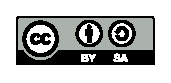
\includegraphics[width = 0.3\textwidth]{pic/CC-BY-SA/BY-SA.eps}
\end{center}

本文档采用 \LaTeX 撰写。这意味着作者在撰写本文档内容的同时还撰写了一份软件源代码,以处理本文档内容的排版、渲染等问题。

“CC-BY-SA 4.0 协议”具有对由\href{https://www.fsf.org/}{自由软件基金会(Free Software Foundation, Inc)}提供的“\href{https://www.gnu.org/licenses/gpl-3.0.html}{GNU GENERAL PUBLIC LICENSE Version 3}”(以下简称“GPLv3协议”)的单向兼容性。这意味着如果您希望在本书的 \TeX 代码的基础上进行再创作和分发,您亦可遵循“GPLv3协议”。在中国大陆,由工业和信息化部信息化和软件服务业司指导,挂靠在中国电子技术标准化研究院的\href{https://www.coscl.org.cn/}{中国开源云联盟(COSCL)},撰写了“\href{https://license.coscl.org.cn/MulanPubL-2.0/index.html}{木兰公共许可证,第2版}”(以下简称“MulanPubL-2.0协议”)。其具有与“GPLv3协议”相似的特性,并对中华人民共和国的法律术语进行了针对性说明。您亦可以根据自己的需要,在本书的 \TeX 代码的基础上进行再创作和分发时,选择使用“MulanPubL-2.0协议”进行分发。

请注意,上述说明基于“CC-BY-SA 4.0 协议”本身的兼容性,不代表本文档的代码采用“GPLv3协议”或“MulanPubL-2.0协议”进行授权或分发。

对于不同协议,作者的建议大致如下:

\begin{itemize}
    \item 如果您希望使用本文档的内容或者文件本身(即代码编译后的二进制文件,包括但不限于.pdf,.ps,.div等格式),遵循“CC-BY-SA 4.0 协议”是更好的选择;
    
    \item 如果您希望在 \TeX 代码(包括但不限于.tex,.sty等格式)的基础上进行再创作和分发,遵循“GPLv3协议”或“MulanPubL-2.0协议”是更好的选择。
\end{itemize}

本声明的最终解释权属于作者。

% 前言

\newpage
\section*{前言}

“概率论与随机过程”是北京邮电大学计算机类学生在大二秋季学期的“二选一”课程之一。这门课程对于数据科学、深度学习等方向的后续学习都十分重要。

在北京邮电大学,该课程的教材是由理学院数学系张丽华副教授和周清教授编纂的《\textit{Probability and Stochastic Processes}》。由于在大部分学校,随机过程都是单独开课,且北邮所使用的教材是本校自编的英文教材,导致课程学习资料匮乏。考虑到本课程的重要意义,作者希望将学习过程的习题解法加以整理,以期惠及后人。

为了方便读者反馈,改进本文档内容,用于生成本文档的 \TeX 代码会被托管在 GitHub 网站上的 \href{https://github.com/itdevwu/BUPT-Probability-and-Stochastic-Processes}{itdevwu/BUPT-Probability-and-Stochastic-Processes} 这一 repo 中。读者可以通过提 issue 和 pull request 等方式来参与到本文档的编修工作中。

受限于作者的知识水平和细致程度,本文档无法做到尽善尽美。恳请各位斧正。

% 水平方向靠右侧对齐
\begin{flushright}
    % 竖直方向靠下对齐
    \vfill \textit{
        北京邮电大学\\
        \theauthor
    }
\end{flushright}


% 目录

\newpage
\section*{目录}
\vspace{-3cm}
\tableofcontents
